%% The following is a directive for TeXShop to indicate the main file
%%!TEX root = diss.tex

\chapter{Solutions}
\label{ch:Solutions}

Having discussed the various fields of study related to augmentation of metadata in \autoref{ch:RelatedWork}: Related Work and a number of algorithms in \autoref{ch:Preliminaries}: Preliminaries, we now explain the algorithms for augmenting metadata. Each of the algorithms takes an input base table and a set of potentially related tables, and outputs a tuple $(\textit{Base-Table}, \textit{Tags-Set})$ as well as a set of tuples:
\[
(\textit{Table-Name},\textit{Tags-Set})
\]
where $\textit{Table-Name}$ is the name of a table related to $\textit{Base-Table}$ and $\textit{Tags-Set}$ is the set of augmented tags for the table. The tags of each table in the set are normalized with respect to each other.


All four algorithms use the existing metadata to help augment additional tags, since we assumed that each table already contains some metadata describing the contents of the table. Two of the four algorithms serve as the baseline, one algorithm is our proposed algorithm, and the final algorithm is modified based on the proposed algorithm to improve performance. Each of the four algorithms compares data instances and augments metadata in different ways. In the next section, we discuss a common procedure shared by all four algorithms to achieve normalization of tags. We then explain each of the four algorithms in \autoref{sec:BruteForceApproach} to \autoref{sec:ImprovedIterativeApproach}.

%%%%%%%%%%%%%%%%%%%%%%%%%%%%%%%%%%%%%%%%%%%%%%%%%%%%%%%%%%%%%%%%%%%%%%
\section{Normalization of tags}
\label{sec:CommonProcedureForNormalizationOfTags}

\begin{figure}
    \centering
    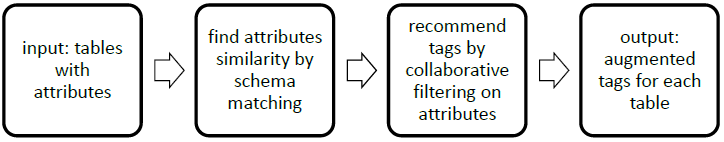
\includegraphics[width=5in]{figures/brute-force-algorithm.png}
    \caption{Brute Force algorithm for metadata tags augmentation}
    \label{fig:brute-force-algorithm}
\end{figure}

\begin{figure}
    \centering
    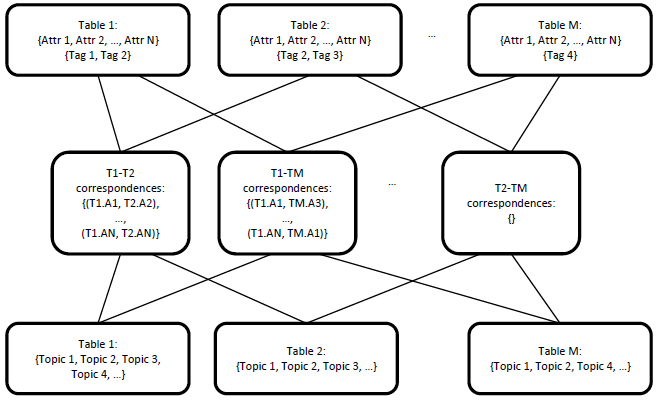
\includegraphics[width=5in]{figures/an-example-instance-brute-force.png}
    \caption{An example instance of tags augmentation by Brute Force}
    \label{fig:an-example-instance-brute-force}
\end{figure}

%\footnote{RAP: this paragraph is new; please check}
As introduced in Section~\ref{sec:intro:normalizing}, if there are two tags describing the same information, the user 
would likely want to add both tags to the metadata of all the tables containing this information. We seek all such tags, and ensure each table contains all the tags describing
the same information. We call this procedure \textit{normalization} of metadata tags. In
other words, a tag is added to all the relevant tables.


%\footnote{RAP: This paragraph has been rewritten. Please check} 
Consider the case there there are two tables, $TABLE_A$ and $TABLE_B$, that we know through some way (e.g., either through asking the users or through the methods described about schema matching) contain much of the information. Then, logically, we would want to see if we could augment the tags of $TABLE_A$ with some of the tags from $TABLE_B$. We call the tags of $TABLE_A$ and $TABLE_B$ $A$ and $B$ respectively. In other words we want to augment $A$ with some of the tags in $B-A$ and augment $B$ with some of the tags in $A-B$. Let the augmented sets of tags be called $A*$ and $B*$ respectively.

The overlap $\textit{A*}\cap\textit{B*}$ contains $A\cap B$; i.e., the number of tags that $TABLE_A$ and $TABLE_B$ have in common will increase. 

Normalization produces the augmented sets \textit{A*} and \textit{B*} by comparing the sets $A$ and $B$ with each other, regardless of the algorithm used. 


%\footnote{RAP: the rest of this subsection is very hard to follow, and I'm not sure that it adds to the reader's understanding. I suggest removing it.} The reason is that $A$ and $B$ are the only sources that the tags originate from. Suppose that there is a third set $C$ which contains all the tags in $A$ and $B$, then $A$ and $B$ do not need to compare to each other. The two sets can use the same criterion to compare to $C$ to obtain \textit{A*} and \textit{B*}. If $A$ and $B$ are initially empty, then the criterion can be created ahead of time, and the tags selected to each set will be normalized with respect to each other. However, if $A$ and $B$ are initially nonempty, then the criterion cannot be created without knowing the existing tags in $A$ and $B$, because the context of use for a tag may be different from the criterion\textquoteright s assumption.

%Using a real world example, let $A$=\ensuremath{\varnothing}, $B$=\ensuremath{\varnothing}, and $C$=\{\textit{park}, \textit{parkland}\}. The table of $A$ is created by one author, while the table of $B$ is created by another. Both tables contain data about \textit{parks} in a city. The two authors then agree that the two tables contain similar data, and therefore both $A$ and $B$ should contain \{park, parkland\}, without the need to examine $A$ and $B$ first. On the other hand, if $A$=\{\textit{park}\}, $B$=\{\textit{parkland}\}, and $C$=\{\textit{park}, \textit{parkland}\}, then the two authors need to examine $A$ and $B$ in order to reach a consensus. The consensus is that both the tags park, parkland are able to describe both tables, which becomes the criterion for adding the tags to another table $D$ containing data about \textit{parks} in a city as well. This example can be generalized to $n$ tables with tags $A_1, A_2, \dots A_n$. 

%We note that this procedure for comparing tables and tags is required for all algorithms that assumes each table\textquoteright s tags set is nonempty.

%%%%%%%%%%%%%%%%%%%%%%%%%%%%%%%%%%%%%%%%%%%%%%%%%%%%%%%%%%%%%%%%%%%%%%
\section{Brute force approach}
\label{sec:BruteForceApproach}

We first explain an algorithm we call Brute Force, which serves as a baseline algorithm. The algorithm is adapted from \cite{Smith2011Unity}, which we briefly explained in \autoref{ssec:ClusteringToReduceComplexity}. The algorithm consists of two separate steps, schema matching and collaborative filtering. Schema matching takes as input two sets of attributes for each pair of tables, and finds a set of correspondences between them. We enforce the one-to-one cardinality constraint between every pair of schemata. Collaborative filtering is then performed to recommend additional tags for each table. We adapted collaborative filtering from \cite{conf/esws/EllefiBDT16}, which was explained in \autoref{ssec:RecommendationOfSimilarDataUsingDataLinking}. For each table $A$, based on the similarity of its attributes with another table(s) $B$, the tags from $B$ are added to $A$'s tags set. If $A$ and $B$ share many similar attributes as determined by attribute correspondences, their tags sets should also be similar. The rule is parameterized by $k$ and $i$: when $A$ and $B$ share $k$ similar attributes, then they should share the subset $i$ of tags. We made a simplification of collaborative filtering by restricting $B$ to be a single table only.

We use \autoref{fig:example-parks} and \autoref{fig:example-park-specimen-trees} as an example. Let $A$ be \textit{Park} and let $B$ be \textit{ParkSpecimenTrees}. Suppose that the tags set of \textit{Park} is \{\textit{parks}\} and the tags set of \textit{ParkSpecimenTrees} is \{\textit{trees}\}. Comparing between \textit{Park.park\_name} and \textit{ParkSpecimenTrees.park} using the N-gram matching criterion yields a similarity score of 0.39. If the threshold is 0.3 and there are no other cardinality constraints, then this pair of attributes forms a correspondence (\textit{Park.park\_name}, \textit{ParkSpecimenTrees.park}, \textit{0.39}). If we suppose that $k$=1 and the subset $i$ is all tags in the tables, then the augmented set of tags for both tables is \{\textit{parks}, \textit{trees}\}.

Given a set of attribute correspondences in \cite{Smith2011Unity}, clustering is then performed to find groups of similar attributes, and each group is labeled with a tag. By performing clustering, a \textit{holistic view} of attribute groups can be obtained. Most existing schema matching algorithms only work well when matching a smaller number of schemata in the repository without obtaining a holistic view. In \cite{10.1145/2396761.2398468}, they used a statistical approach to find a unified model that generates matchings given a number of input schemata. Although a holistic view can be obtained, scalability issues arise due to the need to enumerate all possible models when there are too many schemata in a repository.

A holistic schema matching algorithm is proposed in \cite{Rahm2016Case}, where they first performed pairwise matching between all pairs of schemata, and then clustered the correspondences. The conclusion from a holistic view is that all attributes in the same cluster are highly similar according to some matching criteria. Note that the algorithm does not take into account a base table, which suggests that the output is not optimized for the base table. We replaced clustering with collaborative filtering. When $A$ is the base table, it will be compared with every other table so that tags from any of these tables can be added to $A$'s set. Although there may be too many tags added to the base tables set, we argue that increasing recall while sacrificing precision is a reasonable tradeoff. Normalization of tags can be achieved by assuming each table's tags set is nonempty.

\subsection{The issue with the number of comparisons}

The Brute Force algorithm has the issue of high computational cost due to schema matching performed on all table pairs. For a large number of tables, the number of pairwise attribute comparisons grows exponentially relative to the number of tables and the number of attributes in each table. For example, for $M$ tables and $N$ attributes, the number of comparisons is $C(M,2)\cdot(N\cdot N)$. When there are 100 tables, each with 3 attributes, then there are 44,550 comparisons.

%%%%%%%%%%%%%%%%%%%%%%%%%%%%%%%%%%%%%%%%%%%%%%%%%%%%%%%%%%%%%%%%%%%%%%
\section{Data driven approach}
\label{sec:DataDrivenApproach}

We describe our second baseline algorithm, modified based on \cite{10.1145/3184558.3191601} and briefly explained in \autoref{ssec:SupervisedLearningForSchemaLabeling}. We call the algorithm `Data Driven'. A multiclass classifier is learned from data. Using the classifier, each attribute of a table is assigned a tag (i.e., a class) from a known vocabulary. At the end of Data Driven, the tags assigned to attributes of a table become the augmented tags. We provide as many tables as there are in the repository to the classifier, so that the tags set of every table in the repository is augmented.

The classifier uses a number of matching criterion to compute the similarity score between an attribute and a candidate tag. The hybrid score is computed by combining the scores of each criterion, as discussed in \autoref{ssec:VariationsOfSchemaMatching}. For the pair of attribute and tag with the highest weighted score, the tag becomes the class for the attribute. To train the classifier, we train a weight for each combination of a matching criterion and a tag. The weights are represented as a matrix W, where each row are weights for single tag and each column are weights for a single matching criterion. The supervised learning takes as input a set of pairs of attribute and tag, defined as:
\[
(A_{si},L_{sj})\text{ for }A_{si}\in A_{s},L_{sj}\in L_{s},s\in D'
\]
where the attributes $A_s$ and tags $L_s$ originate from a table $s$ in a set ${D'}$. The set of all tags in the training data is $L$.

For every attribute $A_{si}$ , we create a similarity matrix for pairwise comparisons between the attribute and a tag $L_j$ using matching criterion $M_t$. The similarity matrix is multiplied with the matrix of weights, and the weighted similarity score is compared with the true label in the training data. The losses are used to adjust the weight of a matching criterion relative to other matching criteria. For each example $A_{sj}$ and for each class $L_i$ , the following is the loss: 
\[
\sum_{j}(l(L_{i},A_{sj})-\sum_{t}s(L_{i}|A_{sj},M_{t})\ast W_{M_{t}}^{L_{i}})^{2}
\]
where $l(L_{i},A_{sj})$ is the true label. It is 1 when $L_{i}$ is the class for $A_{sj}$ and 0 otherwise. $s(L_{i}|A_{sj},M_{t})$ is the similarity score the matching criterion $M_{t}$ produces, and $W_{M_{t}}^{L_{i}}$ is the weight for class $L_{i}$ and matching criterion $M_{t}$. The weight of each classifier is adjusted for each training pair $(A_{sj}, L_{i})$ once the accuracy of each matching criterion is computed in the loss function. A weight for a class $L_{i}$ for the $M_{t}$ matching criterion indicates the strength of $M_{t}$ at correctly predicting an attribute $A_{sj}$ to be in the class $L_{i}$.

Note that a limitation of Data Driven is that each attribute is assigned with a single tag only, so the maximum number of new tags augmented is the number of attributes of the table. In addition, the normalization assumes each table's tags set is empty. Our implementation is modified based on the FlexMatcher package provided by the BigGorilla project \cite{DBLP:journals/debu/ChenGHTD18}.

\subsection{Example of multiclass classification}

To show how to augment the tags set of a table using multiclass classification, let the test data be the \textit{Parks} table in \autoref{fig:example-parks}. Let \{\textit{parks}, \textit{environment}, \textit{nature}, \textit{green}, \textit{trees}, \textit{devices}, \textit{infrastructure}\} be the complete set of tags $L$. Let the matching criteria, $M$, be \{\textit{N-gram}, \textit{WordNet}, \textit{FastText}\} for hybrid matching.

Let the trained weights, $W$, of the matching criteria be:

\begin{table}[h!]
    \begin{center}
      \begin{tabular}{|l|l|l|l|l|l|l|l|}
        \hline        
        & \text{N-gram} & \text{WordNet} & \text{FastText}\\
        \hline
        \textit{parks} & 0.3 & 0.4 & 0.3 \\
        \hline
        \textit{environment} & 0.2 & 0.35 & 0.45 \\
        \hline
        \textit{\dots} &  &  &  \\
        \hline
        \textit{infrastructure} & 0.7 & 0.2 & 0.1 \\
        \hline    
      \end{tabular}
    \end{center}
\end{table}

Hybrid matching uses each criterion to compute the similarity score between an attribute and each of the candidate tags. For the attribute \textit{park name} in \textit{Parks}, let the similarity matrix be:

\begin{table}[h!]
\centering	
    \begin{center}
      \begin{tabular}{|l|l|l|l|l|l|l|l|}
        \hline
        & \textit{parks} & \textit{environment} & \textit{nature} & \textit{green} & \textit{trees} & \textit{devices} & \textit{infrastructure}\\
        \hline
        \text{N-gram} & 0.6 & 0.2 & 0.3 & 0.3 & 0.2 & 0.5 & 0.3 \\
        \hline
        \text{WordNet} & 0.8 & 0.6 & 0.6 & 0.6 & 0.5 & 0.2 & 0.2 \\
        \hline
        \text{FastText} & 0.8 & 0.8 & 0.7 & 0.7 & 0.7 & 0.2 & 0.3 \\
        \hline    
      \end{tabular}
    \end{center}
\end{table}

For example, the similarity of (\textit{park name}, \textit{parks}) is 0.6 with N-gram, 0.8 with WordNet, and 0.8 with FastText. Then the combined score is 0.6*0.3 + 0.8*0.4 + 0.8*0.3 = 0.74. In the same way, the combined scores for other candidate tags are (\textit{park name}, \textit{environment}, \textit{0.61}), (\textit{park}, \textit{green}, \textit{0.6}), and so on. If (\textit{park name}, \textit{parks}) has the highest score of 0.74, then the attribute \textit{park name} is assigned to \textit{park}. At the end of Data Driven, the \textit{Parks} table is augmented with \textit{parks} in its tags set.

%%%%%%%%%%%%%%%%%%%%%%%%%%%%%%%%%%%%%%%%%%%%%%%%%%%%%%%%%%%%%%%%%%%%%%
\section{Iterative approach}
\label{sec:IterativeApproach}

We now explain an algorithm that iteratively augments metadata tags given a base table. The output is a set of tables related to the base table, where the base table and each of the related tables contains a normalized tags set. The iterative approach uses the existing small number of tags in tables in the repository, and augments a subset of tables in the repository with additional tags to make their metadata more complete. The subset of tables is related to the base table, which is consistent with the scope of augmenting metadata discussed in \autoref{sec:ScopeOfImprovingMetadata}. That is, since it is unnecessary for a user to look at all tables in the repository, only the tags set of the related tables are augmented. The algorithm emphasizes the process of normalization, such that tables containing overlapping information (i.e., in the data domain of some tag) have one or more shared tags.

The algorithm begins with an initialization step, which creates the semantic labeling (discussed in \autoref{sec:SemanticLabeling}) between attributes and tags for all tables in the repository. The initialization step facilitates normalization of the tags. We then apply an iterative method that integrates a table search step (discussed in \autoref{sec:FindingRelatednessBetweenTables}) and a partitioning step (discussed in \autoref{sec:Partitioning}). The table search step helps discover tables related to the base table. Between the base table and a related table, the partitioning step is performed on the set of semantic labels of the related table. Schema matching is performed throughout the algorithm to verify that a pair of items (either attribute or tag) correspond to each other. The iterative method will be explained in \autoref{ssec:IterativeMethod}. Finally, the tags in the partitions are added to each table's metadata, as explained in \autoref{ssec:FromPartitionsToMetadataTags}.

\begin{figure}
    \centering
    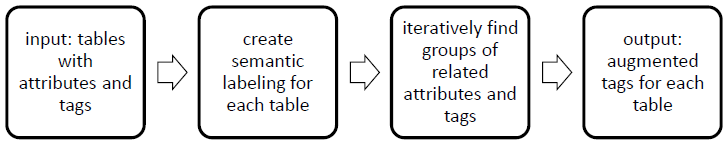
\includegraphics[width=5in]{figures/the-steps-iterative-approach.png}
    \caption{The steps in the iterative approach to augment metadata tags for tables}
    \label{fig:the-steps-iterative-approach}
\end{figure}

\subsection{Semantic labeling as the initialization step}
\label{ssec:SemanticLabelingAsTheInitializationStep}

The iterative method in our algorithm relies on an initialization step, which is performed before the iterative method. The initialization step takes as input a set of attributes and tags $(A_{s},L_{s})$ for each table $s$ in the repository, and a semantic labeling between attributes and tags is found by schema matching (probabilistically as described in \autoref{ssec:UsingSchemaMatchingOnOpenData}). We then take the semantic labels as input, and for the base table, $s_q$, we create empty partitions using the tags in the semantic labels of $s_q$. We create a partition for each topic $L_{j}$ in $s_q$. For each semantic label, $(A_{si},L_{j})$, we place the attribute $A_{si}$ and the tag $L_{j}$ to the sets in the partition of $L_{j}$ as explained in \autoref{ssec:PartitioningSemanticLabels}. We let the set of partitions of table $s_q$ be $S$. $S$ is then compared with the semantic labeling of the other tables in the repository, within table search and partitioning of the iterative method.

With the initialization step, we are able to modify the procedure for comparing two sets for normalization explained in \autoref{sec:CommonProcedureForNormalizationOfTags}. When comparing each pair of sets of tags, the sets have already been  partially normalized. During a preprocessing step, all known tags are collected from the metadata of each table. The set of all tags, $L$, is the vocabulary for all semantic labels and the candidate tags used for augmentation. We assume that the tags already created within a table may be incomplete, but together with tags from all tables, they are sufficient to describe the repository well. When the semantic labeling is performed, we compare a schema attribute with all possible tags instead of just the tags in its own metadata. The semantic labels created have received new tags from other tables, and therefore part of the normalization process has been performed already before the iterative method. The real world analogy is that humans tend to communicate with each other after they are certain what topics will be in the conversation, so that stochasticity in the outcome is reduced.

By performing semantic labeling in the initialization step, we improve the quality of the augmented metadata and the efficiency. The semantic labeling enhances the quality of the related tables retrieved by the table search step, due to the increased tag overlaps between tables. The semantic labels also increase the chance for the partitioning step to correctly place attributes and tags in the correct partition. Another benefit of the initialization step is to facilitate the improvement of the asymptotic computation cost by reducing the pairwise comparisons from exponential (i.e., between all pairs of attributes in Brute Force) to polynomial (i.e., between the tags in an iterative manner), since each table contains more tags for tag comparisons.

\subsection{Iterative method}
\label{ssec:IterativeMethod}

\begin{figure}
  \centering
  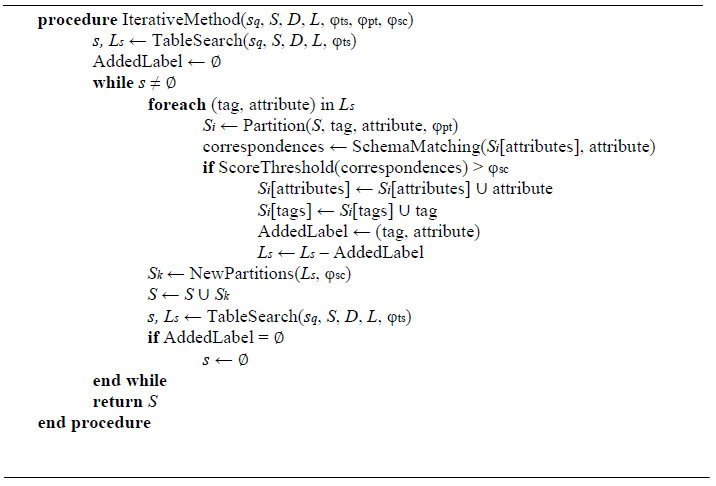
\includegraphics[width=5in]{figures/iterative-method.png}
  \caption{Iterative method}
  \label{fig:iterative-method}
\end{figure}

As proposed by \cite{Smith2011Unity}, to achieve normalization we need to find relationships between the metadata of all tables, and generate additional metadata that captures the relationships to make data more searchable and understandable.

Once we have performed table search and table recommendation, a group of tables is found to be related to a base table, thereby organizing the metadata of the existing tables, and finding relatedness.

Therefore, we need methods to organize the metadata and discover the relatedness.

Our main algorithm uses the table search outlined in \cite{Mudgal2018Deep} to approximate tables that are relevant to the base table.

We emphasize that augmenting metadata is only possible when a group of related tables can be found. A user who manually searches for related tables would encounter the same challenge.

Finding the interesting tags can be achieved by table searching, adopted from \cite{Nargesian2018Table} and \cite{conf/esws/EllefiBDT16}, which we explained in detail in \autoref{ssec:TableSearchOnOpenData} and \autoref{ssec:ModifiedTableSearch}.

Partitioning was explained in \autoref{ssec:PartitioningSemanticLabels}. We explained how we normalize the tags using the semantic labeling, briefly in \autoref{sec:SemanticLabeling}, and more in detail in \autoref{sec:IterativeApproach}. We can iteratively augment metadata of the base table and the tables we retrieved.

After we retrieve one candidate table, we perform schema matching again between the base table and the candidate table in order to augment metadata tags. We use the matched topic pairs from table search to obtain candidate attribute pairs, and then perform attribute-to-attribute schema matching to verify that each pair of attributes belongs to the same domain. For example, given that the overlapping tag is parks, with semantic labeling of (\textit{parks}, \textit{Parks.park\_name}) and (\textit{parks}, \textit{Park\-Specimen\-Trees.park}), we know that the pair of attributes (\textit{Parks.park\_name}, \textit{Park\-Specimen\-Trees.park}) should be compared to verify that they are similar. Once the correspondence between the pair of attributes is confirmed, we can confirm that the tag $parks$ is a correct tag for both tables.

The \textit{iterative method} in \autoref{fig:iterative-method} takes $s_q$, $S$, $D$, $L$, $\ensuremath{\varphi}_{ts}$, $\ensuremath{\varphi}_{pt}$, $\ensuremath{\varphi}_{sc}$ as input, where $D$ is the set of all data instances in the repository, $L$ is the set of text items describing the data instances, $\ensuremath{\varphi}_{ts}$ is a threshold used for schema matching during the table search step, $\ensuremath{\varphi}_{pt}$ is a threshold used for schema matching during the partitioning step, and $\ensuremath{\varphi}_{sc}$ is a threshold used for schema matching during the verification step after items are placed in partitions.

Function \textit{TableSearch} is described in words in \autoref{ssec:ModifiedTableSearch}. We first select a table $s\in D$ that is most closely related to the current state $S$ of $s_q$. The relatedness is determined by the number of overlapping tags between the selected table $s$ and $s_q$. Next, for each semantic label in the selected table, use \textit{Partition} described in \autoref{Partitioning semantic labels} to compare the tag to each partition of $s_q$. Using \textit{Partition}, if the tag is similar to the tags in a partition, then use \textit{SchemaMatching} (described in \autoref{ssec:UsingSchemaMatchingOnOpenData}) to perform schema matching between the tag's mapped attribute and existing attributes in the partition. From \textit{ScoreThreshold}, if correspondences above $\ensuremath{\varphi}_{pt}$ can be created from the result of schema matching, add the tag and the attribute to that partition. If the tag is not highly similar to any tags in any partitions, but the tag is somewhat similar to tags in $s_q$ above a threshold score, then use \textit{NewPartitions} described in \autoref{Partitioning semantic labels} to create a new partition for the tag. Update the current state $S$ to include new partitions and tags. In the selected table $s$, remove tags that were added from its metadata, so that these tags will not overlap with the base table again in the next iteration. Repeat all of the above in a new iteration if it is still possible to find a table $s\in D$ related to the current state $S$ of $s_q$. The only matching criterion we used throughout the algorithm is N-gram.

\subsection{Iterative method example}
\label{ssec:IterativeMethodExample}

We use \autoref{fig:example-parks}, \autoref{fig:example-park-specimen-trees}, etc.~as an example. Let the base table be \textit{ParkSpecimenTrees} with the semantic labeling (\textit{location}, \textit{environment}) and (\textit{tree species}, \textit{trees}), (\textit{park}, \textit{parks}). Let the repository $D$ contain tables \textit{Parks}, \textit{GreenInfrastructureNetwork}, and \textit{DrainageCatchBasins}. We use the semantic labeling in \textit{ParkSpecimenTrees} to search other tables containing the maximum number of overlapping tags. The first table found is \textit{Parks}, with overlapping tags [\textit{environment}, \textit{parks}]. For every tag in \textit{Parks}, we find a partition that it belongs to. Let there be a semantic label (\textit{park\_name}, \textit{parks}) for \textit{Parks}. We compare it with the partition containing the tag \textit{parks}, which also contains \textit{ParkSpecimenTrees.park} in the set of attributes. We then compare the attribute \textit{park} in \textit{ParkSpecimenTrees} with \textit{park\_name} in \textit{Parks}, and find that the two attributes are similar. We add (\textit{park\_name}, \textit{parks}) to the partition, and remove the tag \textit{parks} from the list of tags of \textit{Parks}, so that \textit{parks} will not be an overlapping tag with the base table again in future iterations. After the first iteration, the base table contains tags [\textit{trees}, \textit{parks}, \textit{environment}, \textit{green}, \textit{nature}]. In the second iteration, let the table found be \textit{GreenInfrastructureNetwork} with tags [\textit{ecosystem}, \textit{sustainability}, \textit{green}] and semantic labels \{(\textit{ecological value}, \textit{ecosystem}), (\textit{hub or site}, \textit{green})\}. The base table overlaps with the tag green. By comparing the tags of \textit{GreenInfrastructureNetwork} with partitions in the base table, we find additionally that \textit{ecosystem} is similar to \textit{environment}, and \textit{sustainability} is similar to \textit{environment}. We perform schema matching between attributes of \textit{GreenInfrastructureNetwork} and attributes in the partition of \textit{environment}. Suppose that the correspondence score is above threshold $\ensuremath{\varphi}_{sc}$ for \textit{ecosystem}, and below threshold $\ensuremath{\varphi}_{sc}$ but above 0.5$\ensuremath{\varphi}_{sc}$ for \textit{sustainability}. We add \textit{ecosystem} to the partition containing \textit{environment}. We then create a new partition for \textit{sustainability} by \textit{NewPartitions}. Since there is no semantic label for \textit{sustainability}, the attributes set for the new partition is empty. Once the second iteration completes, the partitions of the base table contain the tags [\textit{trees}, \textit{parks}, \textit{environment}, \textit{green}, \textit{nature}, \textit{ecosystem}, \textit{sustainability}]. These tags are used to find tag overlaps with other tables in the repository, but \textit{Parks} and \textit{GreenInfrastructureNetwork} will not overlap in these tags. In the third iteration, we were unable to find any similar tables and we terminate the iterative method.

We provide a second example with \textit{Parks} as the base table. We find that our base table is similar to \textit{DrainageCatchBasins}, the overlapping tag is \textit{infrastructure}, where the semantic labels are (service \textit{classification}, \textit{infrastructure}) for \textit{Parks} and (\textit{device size}, \textit{infrastructure}) for \textit{DrainageCatchBasins}. After comparing the attributes with \textit{SchemaMatching}, we find that \textit{service classification} and \textit{device size} are not similar, nor is the attribute \textit{device size} similar to any other partitions. Thus we do not add (\textit{device size}, \textit{infrastructure}) to the base table partitions.

\subsection{From partitions to metadata tags}
\label{ssec:FromPartitionsToMetadataTags}

Each partition is a collection containing a set of attributes, a set of tags, and the mapping between attributes and tags. The iterative method takes a set of semantic labeling as input, and outputs the partitions of the base table. We show how to create a modified set of semantic labeling for each table found in \textit{TableSearch}, and how to augment tags of a table using semantic labeling. We let $A(a)$ and $B(b)$ be two tables where $a$ and $b$ are attributes, and let $A$ be the base table. Let tags of $A$ be $[X]$, and tags of $B$ be $[Y]$. Let semantic labeling of $A$ be ${(a, X)}$ and semantic labeling of $B$ be ${(b, Y)}$. Suppose that $X$ and $Y$ are similar, and $a$ and $b$ are similar. Thus there is one partition where the attributes are ${a, b}$ and the tags are ${X, Y}$. We also keep track of the mappings between attributes and tags as well as which table an attribute originates from. For each table, we collect all tags in all partitions where its attributes are assigned, and augment the table tags with any additional tags it does not already contain. For every attribute in a partition, we create a new semantic label for every attribute-tag pair. For example, in addition to the existing semantic labels, the semantic labels $(a, Y)$ and $(b, X)$ are created. Then table $A$ would collect both $X$ and $Y$ as the augmented metadata, and likewise for table $B$.

At the end of the third iteration in the example from \autoref{ssec:IterativeMethodExample}, the augmented tags for \textit{ParkSpecimenTrees} are [\textit{environment}, \textit{ecosystem}, \textit{trees}, \textit{green}, \textit{parks}, \textit{sustainability}], the augmented tags for \textit{Park} are [\textit{environment}, \textit{ecosystem}, \textit{parks}], and the augmented tags for \textit{GreenInfrastructureNetwork} are [\textit{environment}, \textit{ecosystem}, \textit{trees}, \textit{green}].

\begin{figure}
    \centering
    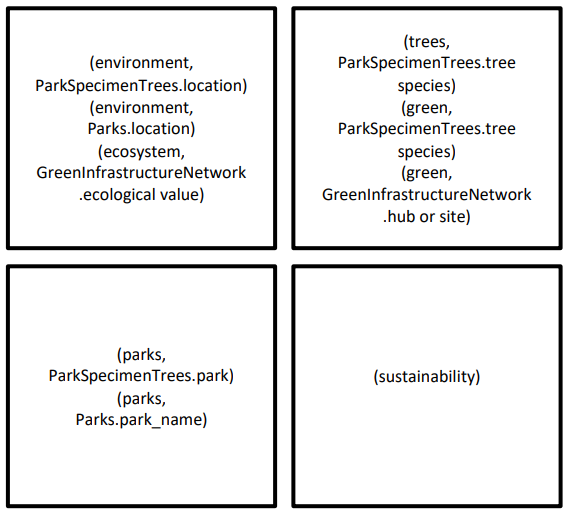
\includegraphics[width=5in]{figures/partitions-park-specimen-trees.png}
    \caption{Partitions of base table \textit{ParkSpecimenTrees} after the third iteration of the example in \autoref{ssec:IterativeMethodExample}. Each partition contains a set of attributes and a set of tags, as well as the mappings between them. They are represented as the set of semantic labels above.}
    \label{fig:partitions-park-specimen-trees}
\end{figure}

%%%%%%%%%%%%%%%%%%%%%%%%%%%%%%%%%%%%%%%%%%%%%%%%%%%%%%%%%%%%%%%%%%%%%%
\section{Improved iterative approach}
\label{sec:ImprovedIterativeApproach}

To perform semantic enrichment, we take the existing table metadata as input, and then create a common representation of information in the form of a list of tags.
With distinct concepts, it is easier to find metadata overlaps.
However, finding distinct concepts requires creating contexts for word sense disambiguation.
Recall that the term \textit{topic} is used for tag with a known dictionary definition and it defines a data domain.
We rely on the semantics of words in the metadata to determine relatedness between data instances.

When metadata are semantically enriched, it is much easier to compare between the metadata and to semantically label attributes with tags. Next, we explain how schema matching uses semantically enriched metadata to effectively label attributes with tags, thus assigning additional context to attributes of a schema.

%We first talk about semantic enrichment and semantic labelling to resolve semantic heterogeneity.

%We first perform semantic enrichment for both attributes and tags, and create semantic labeling between attributes and tags.

The first step is to apply external knowledge such as a domain dictionary to determine the semantics, performed along with word sense disambiguation.
This step performs word sense disambiguation using metadata, and semantically enrich each attribute or tag by associating it with a WordNet Synset.
Since each word used in a tag can have more than one meaning, we attach a dictionary definition to each word in a tag as shown in \autoref{fig:semantically-enriched-attribute}, where we used metadata to disambiguate the words.

Once we disambiguate a word, we are able to identify other words with similar interpretations across all metadata of all tables.

Let us make two changes to Iterative. We name our new algorithm Improved Iterative. The first change is to perform semantic enrichment before semantic labeling during the initialization step. We apply semantic enrichment from \autoref{sec:SemanticLabeling}, where word sense disambiguation is performed on attributes and tags. The second change is to include more matching criteria for schema matching. We use hybrid matching from \autoref{ssec:VariationsOfSchemaMatching} to combine the similarity scores of the different matching criteria.

Enriching metadata relies on the availability of external knowledge, which we can use to assist in resolving conflicting word senses. We create contexts for attributes and tags. We use WordNet as our external knowledge base and the Lesk method discussed in \autoref{sec:SemanticLabeling} to semantically enrich the attributes and tags, and attach the semantics to the attributes and tags. The way that we enrich the attributes and tags is by finding the correct Synset of a word, where the semantics is given. The justification for performing semantic enrichment is that the open data metadata tags and attributes exhibit semantic heterogeneity, and we need to resolve the heterogeneity to allow pairwise comparisons to be effective. If attributes and tags are placed in the same partition, then they must overlap in the data domain, and the attribute names and tag names could be synonyms of each other.

Once semantics is provided by semantic enrichment, we perform schema matching using a matching criterion that assesses the semantic similarity. We chose N-gram as our only matching criterion in Iterative, which we do not think is effective for open data. Improved Iterative combines three matching criteria during schema matching: \textit{N-gram}, \textit{WordNet}, and \textit{FastText}. The weights used to combine the matching criteria are trained by hybrid matching.

\subsection{Initialization step}

As the first step before we perform the initialization step, we perform semantic enrichment (discussed in \autoref{sec:SemanticLabeling}) of attributes and tags for each data instance. For every word $w$ in each attribute $A_{si}$ or tag $L_j$, we perform word sense disambiguation by using gloss overlap between the context of a word sense $C(w)_k$ and the context of the word in the attribute $C(A_{si})_w$ or tag $C(L_j)_w$. The context of a word sense $C(w)_k$ is taken from the domain dictionary $W$. The result comparing a candidate sense with a word is a tuple (\textit{word}, \textit{sense}, \textit{score}), and we select the most likely word sense $C(w)$*, and attach the sense to the word. An example of semantic enrichment of the word \textit{park} is a tuple (\textit{park}, \textit{`a piece of open land for recreational use in an urban area'}).

\subsection{Semantic distance}

Once semantics are attached to each attribute or tag, we can use WordNet to find the semantic distance between two tags, between a tag and an attribute, or between two attributes. The semantic distance can be used in \textit{TableSearch}, \textit{SchemaMatching}, and \textit{NewPartition} in \autoref{fig:iterative-method}, replacing N-gram character matching.

We use hybrid matching \cite{Rahm2001Survey}, where we use each matching criterion to produce a similarity score for each pair of elements compared, and then combine the similarity scores once the scores from all criteria are available. The criteria we use are WordNet semantic distance, FastText word vector distance, and N-gram distance that we described in \autoref{ssec:VariationsOfSchemaMatching}. We reuse the weights of the matching criteria trained in Data Driven, where each trained weight is specific for each tag and each matching criterion. However, the total number of trained weights is $\left|\text{number of tags}\right|\cdot\left|\text{number of criteria}\right|$, which is too costly to compute. We use one score for each criterion instead, where we simply sum up all the weights of all classes for a specific criterion:
\[
\sum_{C_{i}}\ensuremath{W}_{L_{t}}^{C_{i}}
\]

We then normalize the weights such that they sum to 1. For example, when comparing \textit{park} and \textit{trees}, WordNet, FastText, and N-gram each outputs one score, regardless of what tag is being compared. However, we ended up having negative weights for FastText, which means it gave false positives and false negatives during training. On the other hand, the weight of WordNet is twice of N-gram, which indicates that among the three criteria, WordNet performed much better than the other two. We then used the empirical weights of (N-gram=0.4, WordNet=0.6, FastText=0) instead to increase true positives. In the WordNet matching criterion, if an attribute or tag consists of multiple words, we take the maximum of the semantic distance scores.

\subsection{Iterative method example}
\label{ssec:IterativeMethodExample2}

Let the base table schema be \textit{Parks}(\textit{park name}, \textit{location}). Let its existing tags be [\textit{environment}, \textit{green}, \textit{parks}]. After performing semantic enrichment, we have (\textit{park}, \textit{`a piece of open land for recreational use in an urban area'}), (\textit{name}, \textit{`a language unit by which a person or thing is known'}), (\textit{location}, \textit{`a point or extent in space'}), (\textit{environment}, \textit{`the area in which something exists or lives'}), (\textit{green}, \textit{`a piece of open land for recreational use in an urban area'}), (\textit{parks}, \textit{`a piece of open land for recreational use in an urban area'}).

We let a schema in the repository be \textit{PayParkingStations}(\textit{meter station}) and its tags be [\textit{parking station}] with semantics (\textit{meter}, \textit{`any of various measuring instruments for measuring a quantity'}), (\textit{parking}, \textit{`space in which vehicles can be parked'}) and (\textit{station}, \textit{`a facility equipped with special equipment and personnel for a particular purpose'}). We let another schema be \textit{ParkSpecimenTrees}(\textit{park}) and its tags [\textit{parks}] with semantics (\textit{park}, \textit{`a large area of land preserved in its natural state as public property'}) and (\textit{parks}, \textit{`a large area of land preserved in its natural state as public property'}).

After topics of every schemata are collected, we have [\textit{environment}, \textit{green}, \textit{Parks.parks}, \textit{parking station}, \textit{ParkSpecimenTrees.parks}]. We note that two topics may have the same tag name but have different semantics, such as \textit{Parks.parks} and \textit{ParkSpecimenTrees.parks}. We then perform semantic labeling using the semantically enriched attributes and topics. Let the semantic labeling of \textit{Parks} be (\textit{park name}, \textit{Parks.parks}) and (\textit{location}, \textit{environment}), the semantic labeling of \textit{PayParkingStations} be (\textit{meter station}, \textit{parking station}), and the semantic labeling of \textit{ParkSpecimenTrees} be (\textit{park}, \textit{Parks.parks}). We note that \textit{park} from \textit{ParkSpecimenTrees} is labeled with the tag from \textit{Parks}, because the attribute is meant to contain \textit{park names} within a city rather than natural land.

With Park as the base table, we first create 3 partitions for the 3 semantic labels, and apply the iterative method. We use the WordNet semantic distance to find topic overlaps between the base table and a table in the repository. For example, we find the overlap between \textit{Park} and \textit{ParkSpecimenTrees} is \textit{Parks.parks}, and there are no overlapping topics between \textit{Park} and \textit{PayParkingStations}. We proceed to partitioning and schema matching between \textit{Park} and \textit{ParkSpecimenTrees}. We perform comparisons of a candidate topic in \textit{ParkSpecimenTrees} with all the topics in the base table partitions. We find that the candidate topic \textit{Parks.parks} is similar to an existing topic \textit{Parks.parks} in a partition. We now proceed to compare the attribute in the semantic label and all the attributes in the partition. Thus we compare \textit{park} with \textit{park name} using both the N-gram and the WordNet matching criteria. We find that the two attributes are highly similar because the combined score is above a threshold. We note that WordNet compares the word pairs (\textit{park}, \textit{park}) and (\textit{park}, \textit{name}), and takes the higher semantic distance score. We place the candidate topic and the attribute into the partition, now containing topics [\textit{Parks.parks}, \textit{Parks.parks}, \textit{green}] and attributes [\textit{park name}, \textit{park}], where one of the \textit{Parks.parks} is from the \textit{Parks} table and the other is from \textit{ParkSpecimenTrees}.

After the iterative method terminates, the base table and all the related tables are augmented with additional topics from the partitions in the same way as \textit{IterativeMethod}. We note that the resulting topics will be used to compare with a gold standard that we created. We will explain how we compare the augmented topics in our algorithm with the gold standard in \autoref{ssec:ComparingOutputAugmentedTagsWithGoldStandard}.
\endinput